\documentclass[svgnames,11pt]{beamer}
\input{/home/tof/Documents/Cozy/latex-include/preambule_commun.tex}
\input{/home/tof/Documents/Cozy/latex-include/preambule_beamer.tex}
%\usepackage{pgfpages} \setbeameroption{show notes on second screen=left}
\author[]{Christophe Viroulaud}
\title{Graphes\\Représentation carte Course d'Orientation}
\date{\framebox{\textbf{Algo 13}}}
%\logo{}
\institute{Terminale - NSI}

\begin{document}
\begin{frame}
    \titlepage
\end{frame}
\begin{frame}
    \frametitle{}

    \begin{center}
        \centering
        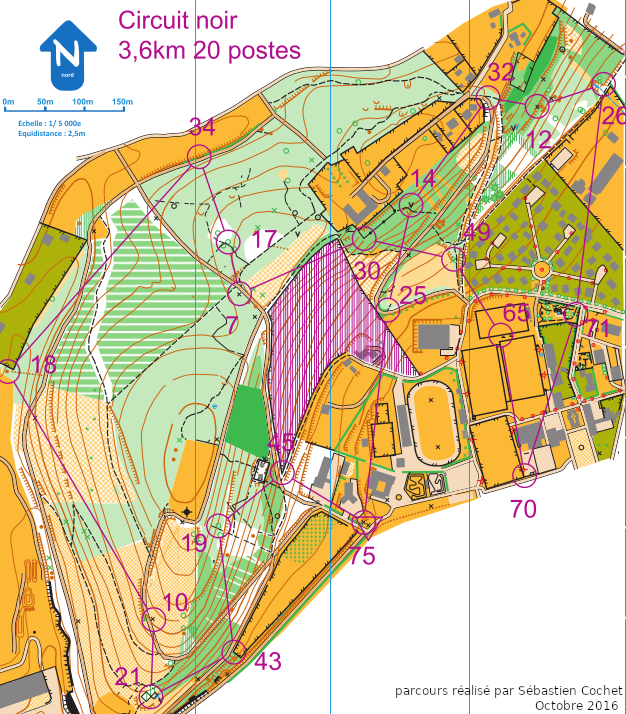
\includegraphics[width=8cm]{ressources/co-noir.png}
    \end{center}
    \note{La course d’orientation est une activité proposée par l’association sportive du lycée. C’est un sport
        très complet et apprécié des élèves. Cependant un inconvénient pour les enseignants qui organisent
        une séance est le temps de préparation nécessaire. Un support numérique peut permettre d’optimiser
        ce temps.}
\end{frame}
\begin{frame}
    \frametitle{}

    \begin{center}
        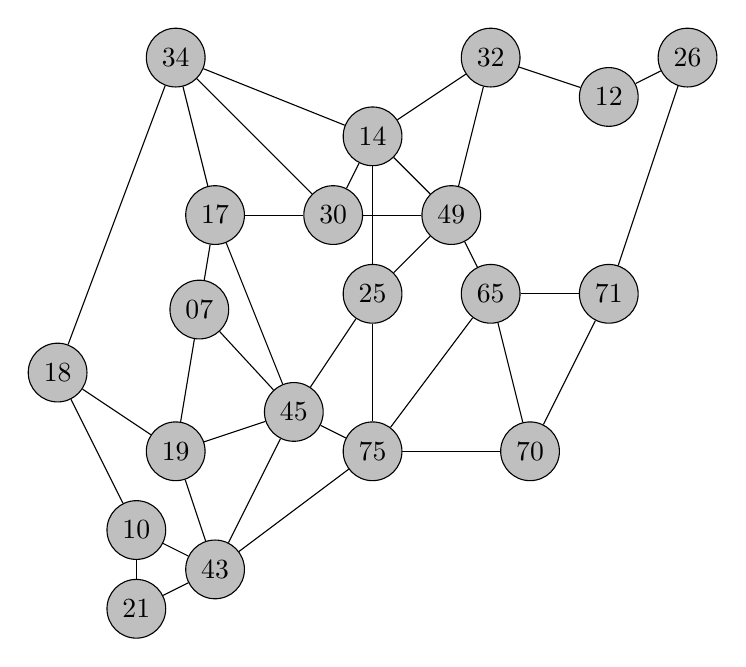
\begin{tikzpicture}
            \node[draw,circle,fill=gray!50] (21)at(0,0) {21};
            \node[draw,circle,fill=gray!50] (43)at(1,0.5) {43};
            \node[draw,circle,fill=gray!50] (10)at(0,1) {10};
            \node[draw,circle,fill=gray!50] (19)at(0.5,2) {19};
            \node[draw,circle,fill=gray!50] (45)at(2,2.5) {45};
            \node[draw,circle,fill=gray!50] (18)at(-1,3) {18};
            \node[draw,circle,fill=gray!50] (75)at(3,2) {75};
            \node[draw,circle,fill=gray!50] (70)at(5,2) {70};
            \node[draw,circle,fill=gray!50] (65)at(4.5,4) {65};
            \node[draw,circle,fill=gray!50] (71)at(6,4) {71};
            \node[draw,circle,fill=gray!50] (25)at(3,4) {25};
            \node[draw,circle,fill=gray!50] (07)at(0.8,3.8) {07};
            \node[draw,circle,fill=gray!50] (17)at(1,5) {17};
            \node[draw,circle,fill=gray!50] (30)at(2.5,5) {30};
            \node[draw,circle,fill=gray!50] (49)at(4,5) {49};
            \node[draw,circle,fill=gray!50] (14)at(3,6) {14};
            \node[draw,circle,fill=gray!50] (34)at(0.5,7) {34};
            \node[draw,circle,fill=gray!50] (32)at(4.5,7) {32};
            \node[draw,circle,fill=gray!50] (12)at(6,6.5) {12};
            \node[draw,circle,fill=gray!50] (26)at(7,7) {26};

            \draw[-,>=latex] (75) -- (45);
            \draw[-,>=latex] (75) -- (25);
            \draw[-,>=latex] (75) -- (65);
            \draw[-,>=latex] (75) -- (70);
            \draw[-,>=latex] (75) -- (43);
            \draw[-,>=latex] (45) -- (07);
            \draw[-,>=latex] (45) -- (43);
            \draw[-,>=latex] (45) -- (25);
            \draw[-,>=latex] (45) -- (19);
            \draw[-,>=latex] (45) -- (17);
            \draw[-,>=latex] (25) -- (14);
            %\draw[-,>=latex] (19) -- (10);
            \draw[-,>=latex] (19) -- (18);
            \draw[-,>=latex] (19) -- (07);
            \draw[-,>=latex] (19) -- (43);
            \draw[-,>=latex] (43) -- (10);
            \draw[-,>=latex] (43) -- (21);
            %\draw[-,>=latex] (43) -- (18);
            \draw[-,>=latex] (10) -- (21);
            \draw[-,>=latex] (10) -- (18);
            \draw[-,>=latex] (34) -- (17);
            \draw[-,>=latex] (70) -- (71);
            \draw[-,>=latex] (70) -- (65);
            \draw[-,>=latex] (49) -- (65);
            \draw[-,>=latex] (49) -- (25);
            \draw[-,>=latex] (49) -- (14);
            \draw[-,>=latex] (49) -- (30);
            \draw[-,>=latex] (49) -- (32);
            \draw[-,>=latex] (30) -- (14);
            \draw[-,>=latex] (30) -- (34);
            \draw[-,>=latex] (30) -- (17);
            \draw[-,>=latex] (14) -- (34);
            \draw[-,>=latex] (14) -- (32);
            \draw[-,>=latex] (32) -- (12);
            \draw[-,>=latex] (12) -- (26);
            \draw[-,>=latex] (65) -- (71);
            \draw[-,>=latex] (71) -- (26);
            \draw[-,>=latex] (18) -- (34);
            \draw[-,>=latex] (07) -- (17);

        \end{tikzpicture}
    \end{center}

\end{frame}
\begin{frame}
    \frametitle{}

    \begin{framed}
        \centering Comment représenter un graphe en mémoire?
    \end{framed}

\end{frame}
\section{Notion de graphe}
\begin{frame}
    \frametitle{Notion de graphe}

    Un graphe est défini par:
    \begin{itemize}
        \item ses \textbf{sommets} (ou \textbf{nœuds}),
        \item ses \textbf{arêtes} (ou \textbf{arcs}) qui relient deux sommets.
    \end{itemize}

\end{frame}
\subsection{Vocabulaire}
\begin{frame}
    \frametitle{Vocabulaire}

    \begin{aretenir}[]
        \begin{itemize}
            \item L'\textbf{ordre} du graphe est le nombre de ses sommets.
            \item Un graphe est \textbf{non orienté} quand ses arêtes peuvent être parcourues dans les deux sens.
        \end{itemize}
    \end{aretenir}
    \begin{center}
        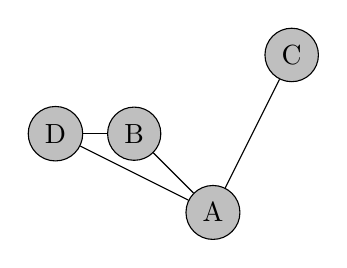
\begin{tikzpicture}
            \node[draw,circle,fill=gray!50] (A)at(1,0) {A};
            \node[draw,circle,fill=gray!50] (B)at(0,1) {B};
            \node[draw,circle,fill=gray!50] (C)at(2,2) {C};
            \node[draw,circle,fill=gray!50] (D)at(-1,1) {D};

            \draw[-,>=latex] (A) -- (B);
            \draw[-,>=latex] (A) -- (C);
            \draw[-,>=latex] (A) -- (D);
            \draw[-,>=latex] (B) -- (D);

        \end{tikzpicture}
        \captionof{figure}{Graphe non orienté d'ordre 4}
    \end{center}
\end{frame}
\begin{frame}
    \frametitle{}

    \begin{aretenir}[]
        \begin{itemize}
            \item<1-> Deux sommets reliés par une arête sont \textbf{adjacents}.
            \item<2-> Le \textbf{degré d’un sommet} est le nombre d’arêtes de ce sommet.
        \end{itemize}
    \end{aretenir}
    \begin{center}
        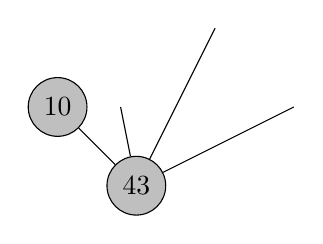
\begin{tikzpicture}
            \node[draw,circle,fill=gray!50] (43)at(1,0) {43};
            \node[draw,circle,fill=gray!50] (10)at(0,1) {10};
            \draw[-,>=latex] (10) -- (43);
            \draw[-,>=latex] (0.8,1) -- (43);
            \draw[-,>=latex] (2,2) -- (43);
            \draw[-,>=latex] (3,1) -- (43);

        \end{tikzpicture}
    \end{center}
\end{frame}
\begin{frame}
    \frametitle{}

    \begin{aretenir}[]
        Un graphe est \textbf{complet} si tous les sommets sont adjacents à tous les autres.
    \end{aretenir}

    \begin{center}
        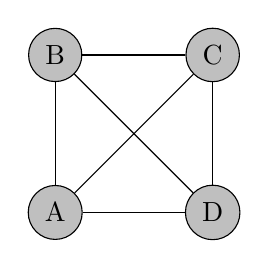
\begin{tikzpicture}
            \node[draw,circle,fill=gray!50] (A)at(0,0) {A};
            \node[draw,circle,fill=gray!50] (B)at(0,2) {B};
            \node[draw,circle,fill=gray!50] (C)at(2,2) {C};
            \node[draw,circle,fill=gray!50] (D)at(2,0) {D};


            \draw[-,>=latex] (A) -- (B);
            \draw[-,>=latex] (A) -- (C);
            \draw[-,>=latex] (A) -- (D);
            \draw[-,>=latex] (B) -- (D);
            \draw[-,>=latex] (B) -- (C);
            \draw[-,>=latex] (C) -- (D);

        \end{tikzpicture}
        \captionof{figure}{Graphe complet d'ordre 4}
    \end{center}
\end{frame}
\subsection{Propriétés}
\begin{frame}
    \frametitle{Propriétés}

    \begin{aretenir}[]
        La somme des degrés d'un graphe est pair.
        $$\sum_{s\in S}{deg(s)}=2.A$$
    \end{aretenir}
    \begin{center}
        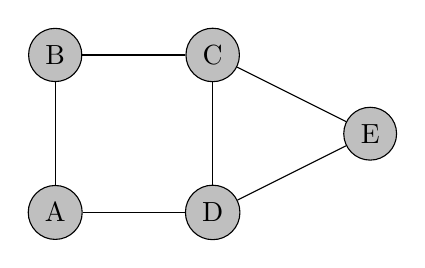
\begin{tikzpicture}
            \node[draw,circle,fill=gray!50] (A)at(0,0) {A};
            \node[draw,circle,fill=gray!50] (B)at(0,2) {B};
            \node[draw,circle,fill=gray!50] (C)at(2,2) {C};
            \node[draw,circle,fill=gray!50] (D)at(2,0) {D};
            \node[draw,circle,fill=gray!50] (E)at(4,1) {E};


            \draw[-,>=latex] (A) -- (B);
            \draw[-,>=latex] (A) -- (D);
            \draw[-,>=latex] (B) -- (C);
            \draw[-,>=latex] (C) -- (D);
            \draw[-,>=latex] (C) -- (E);
            \draw[-,>=latex] (E) -- (D);

        \end{tikzpicture}
        \captionof{figure}{Chaque arête est comptée deux fois.}
    \end{center}
    \note{    Une conséquence est que le nombre de sommets de degré impair est forcément pair (pour avoir somme pair)   }
\end{frame}
\begin{frame}
    \frametitle{}
    \begin{aretenir}[]
        Un arbre est un graphe qui ne possède pas de cycle.
    \end{aretenir}
    \begin{multicols}{2}
        \begin{center}
            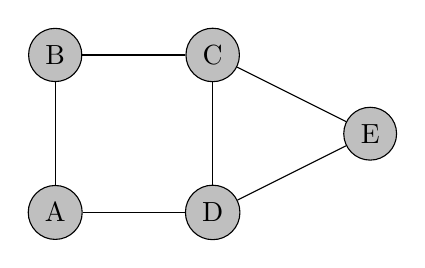
\begin{tikzpicture}
                \node[draw,circle,fill=gray!50] (A)at(0,0) {A};
                \node[draw,circle,fill=gray!50] (B)at(0,2) {B};
                \node[draw,circle,fill=gray!50] (C)at(2,2) {C};
                \node[draw,circle,fill=gray!50] (D)at(2,0) {D};
                \node[draw,circle,fill=gray!50] (E)at(4,1) {E};


                \draw[-,>=latex] (A) -- (B);
                \draw[-,>=latex] (A) -- (D);
                \draw[-,>=latex] (B) -- (C);
                \draw[-,>=latex] (C) -- (D);
                \draw[-,>=latex] (C) -- (E);
                \draw[-,>=latex] (E) -- (D);

            \end{tikzpicture}
            \captionof{figure}{Graphe avec au moins un cycle.}
        \end{center}
        \begin{center}
            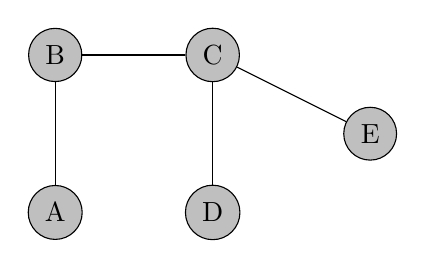
\begin{tikzpicture}
                \node[draw,circle,fill=gray!50] (A)at(0,0) {A};
                \node[draw,circle,fill=gray!50] (B)at(0,2) {B};
                \node[draw,circle,fill=gray!50] (C)at(2,2) {C};
                \node[draw,circle,fill=gray!50] (D)at(2,0) {D};
                \node[draw,circle,fill=gray!50] (E)at(4,1) {E};


                \draw[-,>=latex] (A) -- (B);
                \draw[-,>=latex] (B) -- (C);
                \draw[-,>=latex] (C) -- (D);
                \draw[-,>=latex] (C) -- (E);

            \end{tikzpicture}
            \captionof{figure}{Arbre}
        \end{center}
    \end{multicols}
\end{frame}
\section{Représentations en mémoire}
\subsection{Matrice d'adjacence}
\begin{frame}
    \frametitle{Représentations en mémoire - matrice d'adjacence}
    \begin{aretenir}[]
        La \textbf{matrice d'adjacence} est la représentation mathématique dont le terme $a_{ij}$ vaut 1 si les sommets \emph{i} et \emph{j} sont reliés par une arête et 0 sinon.
    \end{aretenir}
    \begin{multicols}{2}
        \begin{center}
            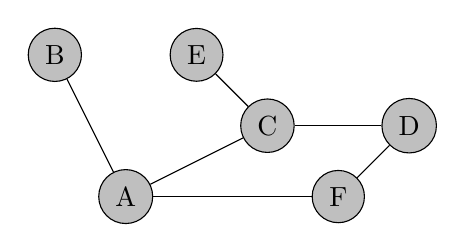
\begin{tikzpicture}[scale=0.9]
                \node[draw,circle,fill=gray!50] (A)at(0,0) {A};
                \node[draw,circle,fill=gray!50] (B)at(-1,2) {B};
                \node[draw,circle,fill=gray!50] (C)at(2,1) {C};
                \node[draw,circle,fill=gray!50] (D)at(4,1) {D};
                \node[draw,circle,fill=gray!50] (E)at(1,2) {E};
                \node[draw,circle,fill=gray!50] (F)at(3,0) {F};
                \draw[-,>=latex] (A) -- (B);
                \draw[-,>=latex] (A) -- (C);
                \draw[-,>=latex] (A) -- (F);
                \draw[-,>=latex] (C) -- (E);
                \draw[-,>=latex] (C) -- (D);
                \draw[-,>=latex] (D) -- (F);
            \end{tikzpicture}
        \end{center}
        $$\begin{pmatrix}
                0 & 1 & 1 & 0 & 0 & 1 \\
                1 & 0 & 0 & 0 & 0 & 0 \\
                1 & 0 & 0 & 1 & 1 & 0 \\
                0 & 0 & 1 & 0 & 0 & 1 \\
                0 & 0 & 1 & 0 & 0 & 0 \\
                1 & 0 & 0 & 1 & 0 & 0 \\
            \end{pmatrix}$$
    \end{multicols}

\end{frame}
\begin{frame}
    \frametitle{}

    \begin{center}
        \begin{tabular}{c|*{6}{c}}
              & A                      & B                       & C                    & D & E & F \\
            \hline
            A & 0                      & \cellcolor{LightGray} 1 & \cellcolor{SkyBlue}1 & 0 & 0 & 1 \\
            B & \cellcolor{LightGray}1 & 0                       & 0                    & 0 & 0 & 0 \\
            C & \cellcolor{SkyBlue}1   & 0                       & 0                    & 1 & 1 & 0 \\
            D & 0                      & 0                       & 1                    & 0 & 0 & 1 \\
            E & 0                      & 0                       & 1                    & 0 & 0 & 0 \\
            F & 1                      & 0                       & 0                    & 1 & 0 & 0 \\
        \end{tabular}
    \end{center}
    \begin{aretenir}[Remarque]
        Dans un graphe non orienté la matrice est symétrique.
    \end{aretenir}
\end{frame}
\begin{frame}
    \frametitle{}

    \begin{activite}
        \begin{enumerate}
            \item Déterminer une structure de données permettant de représenter en mémoire la matrice d'adjacence représentative d'un graphe.
            \item Construire la matrice d'adjacence du graphe suivant:
                  \begin{center}
                      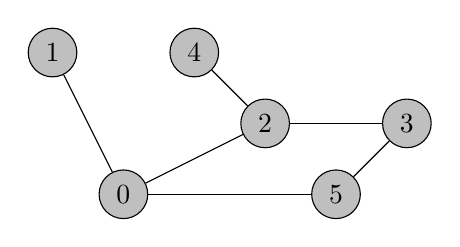
\begin{tikzpicture}[scale=0.9]
                          \node[draw,circle,fill=gray!50] (A)at(0,0) {0};
                          \node[draw,circle,fill=gray!50] (B)at(-1,2) {1};
                          \node[draw,circle,fill=gray!50] (C)at(2,1) {2};
                          \node[draw,circle,fill=gray!50] (D)at(4,1) {3};
                          \node[draw,circle,fill=gray!50] (E)at(1,2) {4};
                          \node[draw,circle,fill=gray!50] (F)at(3,0) {5};
                          \draw[-,>=latex] (A) -- (B);
                          \draw[-,>=latex] (A) -- (C);
                          \draw[-,>=latex] (A) -- (F);
                          \draw[-,>=latex] (C) -- (E);
                          \draw[-,>=latex] (C) -- (D);
                          \draw[-,>=latex] (D) -- (F);
                      \end{tikzpicture}
                  \end{center}
        \end{enumerate}
    \end{activite}

\end{frame}
\begin{frame}[fragile]
    \frametitle{Correction}
    \begin{center}
        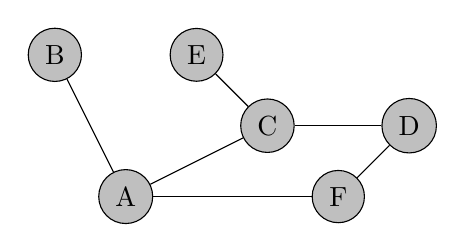
\begin{tikzpicture}[scale=0.9]
            \node[draw,circle,fill=gray!50] (A)at(0,0) {A};
            \node[draw,circle,fill=gray!50] (B)at(-1,2) {B};
            \node[draw,circle,fill=gray!50] (C)at(2,1) {C};
            \node[draw,circle,fill=gray!50] (D)at(4,1) {D};
            \node[draw,circle,fill=gray!50] (E)at(1,2) {E};
            \node[draw,circle,fill=gray!50] (F)at(3,0) {F};
            \draw[-,>=latex] (A) -- (B);
            \draw[-,>=latex] (A) -- (C);
            \draw[-,>=latex] (A) -- (F);
            \draw[-,>=latex] (C) -- (E);
            \draw[-,>=latex] (C) -- (D);
            \draw[-,>=latex] (D) -- (F);
        \end{tikzpicture}
    \end{center}
    \begin{center}
        \begin{lstlisting}[language=Python , basicstyle=\ttfamily\small, xleftmargin=2em, xrightmargin=2em]
# Le noeud A est représenté par la ligne 0
mat = [ [0, 1, 1, 0, 0, 1],
        [1, 0, 0, 0, 0, 0],
        [1, 0, 0, 1, 1, 0],
        [0, 0, 1, 0, 0, 1],
        [0, 0, 1, 0, 0, 0],
        [1, 0, 0, 1, 0, 0] ]
\end{lstlisting}
        \captionof{code}{Tableau de tableau}
        \label{CODE}
    \end{center}

\end{frame}
\begin{frame}
    \frametitle{}

    \begin{aretenir}[Observation]
        Cette représentation peut être gourmande en mémoire: si le nombre d'arêtes est faible, la structure contient peu d'informations. La matrice est \textbf{creuse}.
    \end{aretenir}

\end{frame}
\subsection{Dictionnaire d'adjacence}
\begin{frame}
    \frametitle{Dictionnaire d'adjacence}
    \begin{aretenir}[]
        Un dictionnaire d'adjacence liste les sommets adjacents à chaque sommet.
    \end{aretenir}
    \begin{center}
        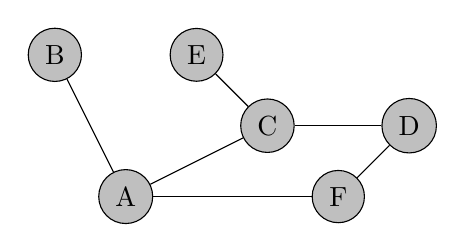
\begin{tikzpicture}[scale=0.9]
            \node[draw,circle,fill=gray!50] (A)at(0,0) {A};
            \node[draw,circle,fill=gray!50] (B)at(-1,2) {B};
            \node[draw,circle,fill=gray!50] (C)at(2,1) {C};
            \node[draw,circle,fill=gray!50] (D)at(4,1) {D};
            \node[draw,circle,fill=gray!50] (E)at(1,2) {E};
            \node[draw,circle,fill=gray!50] (F)at(3,0) {F};
            \draw[-,>=latex] (A) -- (B);
            \draw[-,>=latex] (A) -- (C);
            \draw[-,>=latex] (A) -- (F);
            \draw[-,>=latex] (C) -- (E);
            \draw[-,>=latex] (C) -- (D);
            \draw[-,>=latex] (D) -- (F);
        \end{tikzpicture}
    \end{center}
    \begin{itemize}
        \item A: B, C, F
        \item B: A
        \item C: A, D, E
        \item D: C, F
        \item E: C
        \item F: A, D
    \end{itemize}

\end{frame}
\begin{frame}
    \frametitle{}

    \begin{activite}
    Construire le dictionnaire d'adjacence en Python du graphe suivant:
    \begin{center}
        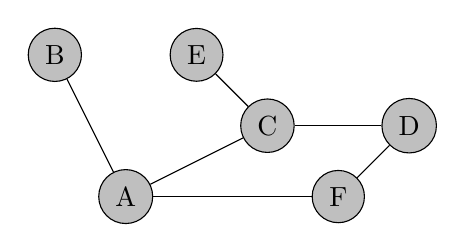
\begin{tikzpicture}[scale=0.9]
            \node[draw,circle,fill=gray!50] (A)at(0,0) {A};
            \node[draw,circle,fill=gray!50] (B)at(-1,2) {B};
            \node[draw,circle,fill=gray!50] (C)at(2,1) {C};
            \node[draw,circle,fill=gray!50] (D)at(4,1) {D};
            \node[draw,circle,fill=gray!50] (E)at(1,2) {E};
            \node[draw,circle,fill=gray!50] (F)at(3,0) {F};
            \draw[-,>=latex] (A) -- (B);
            \draw[-,>=latex] (A) -- (C);
            \draw[-,>=latex] (A) -- (F);
            \draw[-,>=latex] (C) -- (E);
            \draw[-,>=latex] (C) -- (D);
            \draw[-,>=latex] (D) -- (F);
        \end{tikzpicture}
    \end{center}
    \end{activite}

\end{frame}
\begin{frame}[fragile]
    \frametitle{Correction}
    \begin{center}
        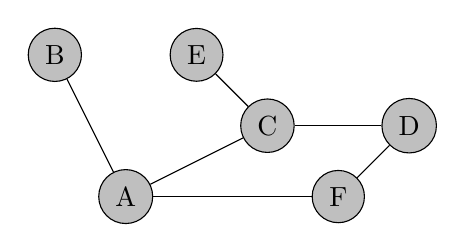
\begin{tikzpicture}[scale=0.9]
            \node[draw,circle,fill=gray!50] (A)at(0,0) {A};
            \node[draw,circle,fill=gray!50] (B)at(-1,2) {B};
            \node[draw,circle,fill=gray!50] (C)at(2,1) {C};
            \node[draw,circle,fill=gray!50] (D)at(4,1) {D};
            \node[draw,circle,fill=gray!50] (E)at(1,2) {E};
            \node[draw,circle,fill=gray!50] (F)at(3,0) {F};
            \draw[-,>=latex] (A) -- (B);
            \draw[-,>=latex] (A) -- (C);
            \draw[-,>=latex] (A) -- (F);
            \draw[-,>=latex] (C) -- (E);
            \draw[-,>=latex] (C) -- (D);
            \draw[-,>=latex] (D) -- (F);
        \end{tikzpicture}
    \end{center}
\begin{center}
\begin{lstlisting}[language=Python , basicstyle=\ttfamily\small, xleftmargin=2em, xrightmargin=2em]
dico = {"A": ["B", "C", "F"],
        "B": ["A"],
        "C": ["A", "D", "E"],
        "D": ["C", "F"],
        "E": ["C"],
        "F": ["A", "D"]}
\end{lstlisting}
\captionof{code}{Dictionnaire de tableau}
\label{CODE}
\end{center}

\end{frame}
\subsection{Passage d'une structure à l'autre}
\begin{frame}
    \frametitle{Passage d'une structure à l'autre}

    \begin{activite}
    Écrire la fonction \textbf{\texttt{mat\_to\_dic(mat: list) $\rightarrow$ dict}} qui construit le dictionnaire d'adjacence à partir de la matrice d'adjacence.\\\underline{Indication:} Les nœuds sont nommés en suivant l'ordre alphabétique majuscule. La première ligne de la matrice représente les adjacences de \textbf{\texttt{A}}. La fonction native \textbf{\texttt{chr(n: int) $\rightarrow$ str}} renvoie le caractère correspondant au point de code UTF-8 \textbf{\texttt{n}}.
    \end{activite}

\end{frame}
\begin{frame}[fragile]
    \frametitle{Correction}

\begin{center}
\begin{lstlisting}[language=Python , basicstyle=\ttfamily\small, xleftmargin=2em, xrightmargin=2em]
def mat_to_dic(mat: list) -> dict:
    dico = {}
    for i in range(len(mat)): 
        # nom du noeud
        noeud = chr(65+i)
        dico[noeud] = []

        for j in range(len(mat[i])):
            if mat[i][j] == 1:
                # noeud adjacent
                adj = chr(65+j)
                dico[noeud].append(adj)
    return dico
\end{lstlisting}
\end{center} 

\end{frame}
\begin{frame}
    \frametitle{}

    \begin{activite}
    Écrire la fonction \textbf{\texttt{dic\_to\_mat(dic: dict) $\rightarrow$ list}} qui construit la matrice d'adjacence à partir de la matrice d'adjacence. \\\underline{Indication:} La fonction native \textbf{\texttt{ord(c: str) $\rightarrow$ int}} renvoie le point de code UTF-8 correspondant au caractère \textbf{\texttt{c}}.
    \end{activite}

\end{frame}
\begin{frame}[fragile]
    \frametitle{Correction}

\begin{center}
\begin{lstlisting}[language=Python , basicstyle=\ttfamily\small, xleftmargin=2em, xrightmargin=2em]
def dic_to_mat(dic: dict) -> list:
    # taille de la matrice connue
    mat = [ [0 for _ in range(len(dic))] 
                for _ in range(len(dic)) ]
    for noeud, adjacents in dic.items():
        # indice de la ligne
        ind_noeud = ord(noeud)-65

        for adj in adjacents:
            # indice de la colonne
            ind_adj = ord(adj)-65
            mat[ind_noeud][ind_adj] = 1
    return mat
\end{lstlisting}
\end{center}

\end{frame}
\subsection{Représentation de la carte de CO}
\begin{frame}[fragile]
    \frametitle{Représentation de la carte de CO}

    \begin{activite}
        L'organisme qui maintient les cartes à jour stocke les informations dans un fichier \textbf{\texttt{json}}. 
        \begin{enumerate}
            \item Télécharger le dossier compressé \textbf{\texttt{representation-co.zip}} et extraire le fichier \textbf{\texttt{parcours\_noir.json}}
            \item Ouvrir le fichier et observer la structure des données.
            \item Créer le fichier \textbf{\texttt{parcours\_noir.py}}
            \item Importer les données \emph{json}.
            \item Créer le dictionnaire d'adjacence associé à la carte de CO de la forme
            \begin{center}
            \begin{lstlisting}[language=Python , basicstyle=\ttfamily\small, xleftmargin=2em, xrightmargin=2em]
{7: [17, 19, 45], 10: [18, 21, 43], 12: [26, 32],...}
\end{lstlisting}
            \end{center}
        \end{enumerate}
    \end{activite}

\end{frame}
\begin{frame}[fragile]
    \frametitle{Correction}

\begin{center}
\begin{lstlisting}[language=Python , basicstyle=\ttfamily\small, xleftmargin=1em, xrightmargin=0em]
import json

f = open("parcours_noir.json")
donnees = json.load(f)  # tableau de dictionnaires
dico_adj = {}
for info in donnees:
    sommet = info["sommet"]
    adjacents = info["adjacents"]
    dico_adj[sommet] = adjacents
f.close()
\end{lstlisting}
\end{center}    

\end{frame}
\end{document}